\newpage
\section{\textit{Layered Label Propagation}}

  A principal ideia dos algoritmos de \textit{Label Propagation} seguem um padrão comum. Estes algoritmos consistem num conjunto de iterações e no início é atribuído a cada vértice uma \textit{label} que representa o \textit{cluster} a que pertence. No início do algoritmo, cada vértice tem uma \textit{label} diferente. O critério de atribuição da \textit{label},a cada vértice, é o que diferencia os vários algoritmos de \textit{Label Propagation}. Um dos algoritmos mais conhecidos é o \textit{Standard Label Propagation}, em que a regra de atribuição da \textit{label} a um vértice é a \textit{label} que ocorrer mais frequentemente na sua vizinhança. 
  
  Uma outra variante, denominada \textit{Absolute Pott Model}, indica que a \textit{label} que é atribuída ao vértice é a que maximiza a seguinte equação: 
 
  \begin{center}
    \begin{equation}
      \label{apmeq}
      ki-\gamma(vi-ki)
    \end{equation}
  \end{center}    
  
  Sendo, $ki$ os vértices na vizinhança que têm a $label_i$ e $v_i$ todos os vértices que têm a $label_i$.
  Este algoritmo pode ser descrito da seguinte forma:
  
  \begin{algorithm}[H]
    \caption{\textit{Absolute Pott Model}}\label{apmalg}
    \begin{enumerate}
    \item Obter uma permutação do grafo.
    \item Iniciar todos os vértices atribuindo uma \textit{label} única e por $v_i=1$ para cada $label_i$ .
    \item Iterar sobre a permutação obtida e para todas as \textit{labels} na vizinhança de cada vértice ver qual é maximizada pela equação \ref{apmeq} e atribuir ao vértice essa \textit{label}. Decrementar $v_i$ para a \textit{label} antiga e incrementar o $v_i$ correspondente à nova \textit{label}.
    \end{enumerate}
  \end{algorithm}

  Ambos os algoritmos apresentados anteriormente têm alguns problemas. O \textit{Standard Label Propagation} tende a produzir um \textit{clusters} de grandes dimensões(contendo a maior parte dos vértices) e o \textit{Absolute Pott Model} tem o problema de não se saber à partida o valor ideal para $\gamma$.
  
  \subsection{Algoritmo de \textit{Layered Label Propagation}}
  Baseado no algoritmo \textit{Standard Label Propagation} surgiu o \textit{Layered Label Propagation}. Este algoritmo consiste no seguinte:
  
  \begin{algorithm}[H]
    \caption{\textit{Layered Label Propagation}}\label{llpalg}
    \begin{enumerate}
    \item Para cada iterações chamar o Algoritmo \ref{apmalg} tendo $gama$ valores compreendidos dentro do seguinte conjunto: $\{0\}\cup\{2^{{-}i},i=0,...,K\} $.
    \item Com o \textit{output} resultante da chamada ao Algoritmo \ref{apmalg}, ordenar os vértices de modo a que os que tenham a mesma \textit{label} fiquem próximos. Para vértices que estejam na mesma comunidade (têm a mesma \textit{label}) é mantida a sua ordem.
    \end{enumerate} 
  \end{algorithm}
  
  \paragraph{Exemplo} Para o grafo da Figura \ref{graph0llp} pode-se calcular 
de forma sequencial o Layered Label Propagation, para cada iteração $i$, 
começando por se fazer uma permutação($\pi_i$) dos vértices do grafo e itera-los 
por essa ordem. 
  
  \begin{figure}[H]
    \center
    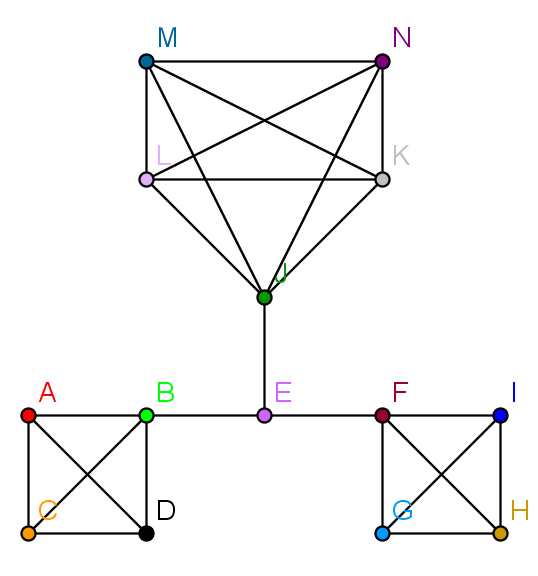
\includegraphics{graph_step0.png}
    \caption{Grafo de exemplo em que cada vértice foi-lhe atribuída uma \textit{label}(cor) inicial que é única.}
    \label{graph0llp}
  \end{figure}
  
  Neste contexto as \textit{labels} serão iteradas de forma a que seja dada uma maior importância à que o vértice tem e de seguida à que pertence ao vértice com menor ordem lexicográfica.

  Para $i=1$ admite-se que $\pi_1=$[N,H,M,B,J,L,G,D,K,E,I,F,C,A], $\gamma=1$(para facilitar) e que $v_i$=1 para todas as \textit{label}. Segundo o algoritmo \ref{apmalg} segue-se a iteração sobre $\pi_1$ e para cada vértice vê-se qual a \textit{label} que maximiza a Equação \ref{apmeq}. 
  %Nesta primeira iteração para qualquer vértice o resultado da equação \ref{apmeq} referente à sua \textit{label} não é o valor que maximiza porque $k_i=0$ e o mesmo acontece para as \textit{labels} que não se encontram na vizinhança, daí a omissão destes elementos. 
  \\[0.25cm]
  Exemplo para N:
  \begin{itemize}
   \item $label_n = k_n - \gamma ( v_n - k_n ) = 0 - 1 ( 1 - 0) = -1$
   \item $label_j = k_j - \gamma ( v_j - k_j ) = 1 - 1 ( 1 - 1) = 1$\\
   {\bf N fica com a \textit{label} de J.}
   \item $label_k = k_k - \gamma ( v_k - k_k ) = 1 - 1 ( 1 - 1) = 1$
   \item $label_l = k_l - \gamma ( v_l - k_l ) = 1 - 1 ( 1 - 1) = 1$ 
   \item $label_m = k_m - \gamma ( v_m - k_m ) = 1 - 1 ( 1 - 1) = 1$
  \end{itemize}
  Este cálculo é feito para todos os vértices pela ordem de $\pi_1$.  \\[0.25cm]
  \begin{figure}[H]
    \center
    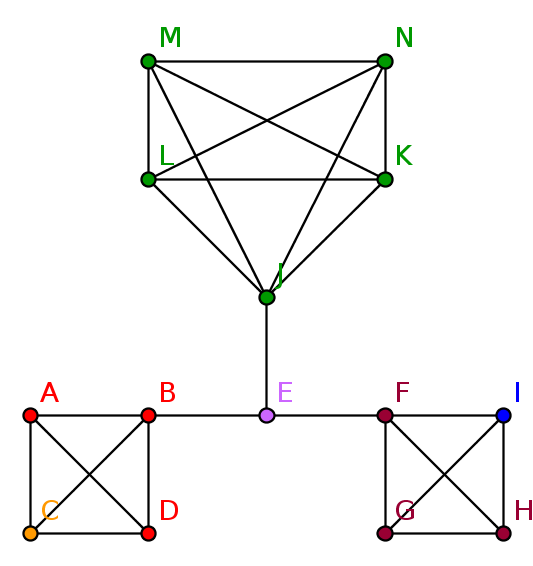
\includegraphics{graph_stepAtE.png}
    \caption{Grafo de exemplo a iterar $\pi_1$ em E}
    \label{graphEllp}
  \end{figure}
  
  Exemplo para E:
  \begin{itemize}
   \item $label_e = k_e - \gamma ( v_e - k_e ) = 0 - 1 ( 1 - 0) = -1$
   \item $label_a = k_a - \gamma ( v_a - k_a ) = 1 - 1 ( 3 - 1) = -1$
   \item $label_f = k_f - \gamma ( v_f - k_f ) = 1 - 1 ( 3 - 1) = -1$ 
   \item $label_j = k_j - \gamma ( v_j - k_j ) = 1 - 1 ( 5 - 1) = -3$\\
   {\bf E mantém a sua \textit{label}.}
  \end{itemize}
  
  No final deste percorrer $\pi_1$ o grafo irá ter 4 comunidades com está 
  apresentado na Figura \ref{graphfinalllp}.
  
  \begin{figure}[H]
    \center
    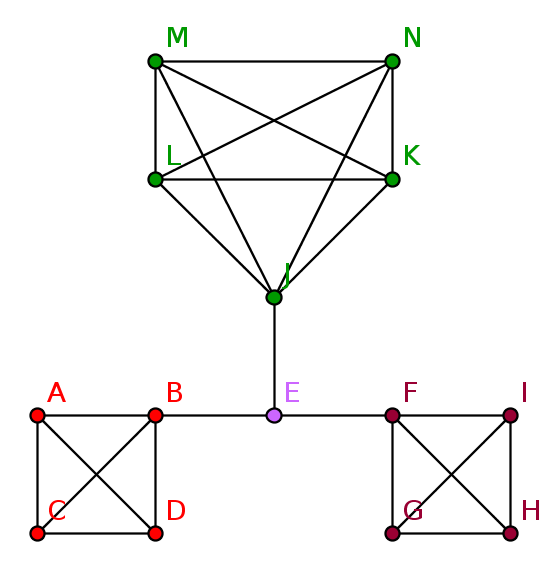
\includegraphics{graph_stepFinal.png}
    \caption{Grafo depois de iterar $\pi_1$ de acordo com o Algoritmo \ref{apmalg}.}
    \label{graphfinalllp}
  \end{figure}
  
  O algoritmo do \textit{Layered Label Propagation} após fazer o algoritmo de
  Absolute Pott Model reordena os vértices de acordo com a sua comunidade 
(mantendo a ordem dos vértices com a mesma comunidade) e volta a fazer este 
processo.

\newpage
\subsection{Algoritmo de \textit{Layered Label Propagation} Distribuído}

O algoritmo apresentado anteriormente pode ser usado em grafos de grandes
dimensões em plataformas distribuídas. Contudo, existe algumas mudanças quanto 
à várias fases do algoritmo. 

  O facto de se estar a usar uma plataforma distribuídas e a ordem que os 
vértices são iterados tem alguma aleatoriedade então a fase de obtenção da 
permutação do vértices é garantida. Após a obtenção da permutação como o 
algoritmo \ref{apmalg} indica, apenas é necessário iterar sobre as 
\textit{labels} que estão na vizinhança. Contudo, é necessário haver uma fase 
de agregação para saber o $v_i$ correto em todos os vértices que têm uma 
determinada $label_i$ de modo a que o valor de $v_i$ não esteja desatualizado 
nas extremidades da comunidade. Para haver essa agregação do $v_i$ há a 
necessidade de cada vértice enviar para o representante da sua comunidade. O 
representante de uma comunidade tem de enviar de volta o valor atualizado de 
$v_i$.

O representante de uma comunidade pode ser um vértice qualquer, isto é, não 
tem de necessariamente, isto permite evitar algumas situações que 
podiam a levar ao aumento da complexidade do algoritmo. Por norma, o 
representante de uma comunidade A é o vértice A.

Para este algoritmo é necessário o uso de mensagens compostas por: vértice de 
origem(quem envia a mensagem), $label_i$ do vértice e $v_i$ conhecido da sua 
$label_i$. Cada vértice tem como valor a sua $label$.

  \begin{algorithm}
    \begin{minipage}{\textwidth}

    \caption{\textit{Layered Label Propagation} 
Distribuído}\label{llpdistributed}
    \begin{enumerate}
     \item Iniciação:
      \begin{enumerate}
       \item Começa-se por atribuir uma \textit{label} única a cada vértice e 
atribuir a essa mesma \textit{label} um $v_i=1$. Inicialmente, cada vértice é 
representante da sua comunidade.
      \end{enumerate}
    \item 1º Passo\footnote{O passos do algoritmo \ref{llpdistributed} ocorrem 
em \textit{supersteps} diferentes entre si.} - Atualização de $v_i$ e propagação 
da $label$.
    \begin{enumerate}
      \item Caso haja mensagens, atualizar o valor de $v_i$ para cada vértice 
com $label_i$. Caso o vértice tenha recebido uma mensagem então escolhe como 
representante quem lhe enviou essa mesma mensagem.
      \item Enviar para os seus vértices adjacentes informação acerca do 
vértice atual.   
    \end{enumerate}
    \item 2º Passo - Cálculo da $label$.
    \begin{enumerate}
      \item Calcular a formula \ref{apmeq} para as $labels$ que recebeu 
e para a sua $label$ atual. Para o cálculo da sua $label$ atual ter em conta 
para o seu $k_i$ o próprio vértice caso tenha recebido mensagens de vértices 
que tenha a mesma $label$. Ver a $label$ que maximiza e em caso 
caso de empate aplicar um método de desempate\footnote{Vai-se aplicar o 
método de desempate que consiste em escolher a \textit{label} menor.}. O método 
de desempate tem de se manter constante para todo o algoritmo.
      \item Se a iteração for par\footnote{Entende-se por uma iterações um 
conjunto de 3 passos do algoritmo. Uma iteração, par ou ímpar, é dada pela 
seguinte expressão: (nº superstep/3) mod 3, em que 0 indica que é uma iteração 
par e 1 uma iteração ímpar.}, não permitir que vértices vão para comunidades 
inferiores à sua.
      \item Enviar para o representante da sua comunidade uma mensagem com a 
informação do vértice. 
      \item Num agregador, agregar o estado se o vértice mudou ou não de 
comunidade. Fazer \textit{halt} ao vértice.
    \end{enumerate}
    \item 3º Passo - Caso esteja ativo neste passo então recebeu 
mensagens, querendo dizer que é representante de uma comunidade. 
    \begin{enumerate}   
    \item Verificar o estado do agregador, se tiver informação que 
todos os vértices não mudaram de comunidade então para-se a computação e 
termina o algoritmo. 
      \item Para todas as mensagem:
      \begin{enumerate}
	\item Calcular $v_i$. O novo $v_i$ é o número de mensagens recebidas no 
representante.
	\item Para iterações ímpares é necessário evitar possíveis 
ciclos\footnote{Dá-se a possibilidade de acontecer ciclos em iterações ímpares 
para que o algoritmo convirja para uma melhor escolha de comunidades.}:
	\begin{enumerate}
	  \item Caso tenha recebido mensagens de um vértice cujo 
$id$ é igual à comunidade atual deste então significa que houve um ciclo. Para 
resolver estes ciclos nos representantes é necessário escolher a $label$ menor 
entre a que tem atualmente e a que recebeu. 
	  \item Devido à escolha de $label$ que é efetuada para resolver ciclos 
neste passo, há a necessidade de ignorar para o cálculo de $v_i$ mensagens 
provenientes de um vértice cujo $id$ é igual à $label$ atual do representante e 
cuja $label$ é superior à $label$ que o representante tem.
	\end{enumerate}
      \end{enumerate}
      \item Escolher o novo representante da comunidade, sendo esse 
representante o vértice que está a calcular o valor de $v_i$ se ele pertencer 
à comunidade. Caso o vértice que está a calcular o novo valor de $v_i$ não 
pertença à comunidade então o novo representante será o vértice com menor 
\textit{id} pertencente à comunidade.
    \end{enumerate}
    \item Repetir a partir do 1º passo.  
    \end{enumerate}
    \end{minipage}
  \end{algorithm}

 \paragraph{Exemplo} Para o grafo da Figura \ref{graph0llp} o \textit{Layered 
Label Propagation} distribuído para o algoritmo \ref{llpdistributed} acontece o 
seguinte:

Fase de Iniciação:
